\documentclass[UTF-8]{ctexart} 
\usepackage[a4paper,left=2cm,right=2cm,top=2.5cm,bottom=2.5cm]{geometry}
\usepackage{amsmath,bm,amssymb}
\usepackage{siunitx}
\usepackage{physics}
\usepackage{lmodern}
\usepackage{tikz}
\usepackage{cutwin}
\usepackage{fancyhdr}
\usepackage{caption}
\usepackage{enumitem}
\usepackage{upgreek}
\usepackage{circuitikz}
\usepackage{mathrsfs}
\usetikzlibrary{snakes,fadings}
\usetikzlibrary{decorations.pathmorphing}
\usetikzlibrary{shapes}
\usetikzlibrary{arrows.meta}

\tikzfading[name=fade left, left color=transparent!30, right color=transparent!70]

\captionsetup{labelformat=empty}
%\renewcommand\thefigure{\theenumi}
\makeatletter
\renewcommand*\maketitle{
    \begin{center}
        \bfseries
        {\Large \@title \par}
        \vskip 1em
        {\global\let\author\@empty}
        {\global\let\date\@empty}
    \end{center}
  \setcounter{footnote}{0}
}
\newcommand{\mlabel}[2]{#2\def\@currentlabel{#2}\label{#1}}
\newcommand{\cube}[5]{
    \pgfmathsetmacro{\cubex}{#2}
    \pgfmathsetmacro{\cubey}{#3}
    \pgfmathsetmacro{\cubez}{#4}
    \filldraw[#5!50,join=round] #1 -- ++(-\cubex,0,0) -- ++(0,-\cubey,0) -- ++(\cubex,0,0) -- cycle;
    \filldraw[#5,join=round] #1 -- ++(0,0,-\cubez) -- ++(0,-\cubey,0) -- ++(0,0,\cubez) -- cycle;
    \filldraw[#5!80,join=round] #1 -- ++(-\cubex,0,0) -- ++(0,0,-\cubez) -- ++(\cubex,0,0) -- cycle;
}
\renewcommand\theenumi{S-\arabic{enumi}}
\renewcommand\labelenumi{\theenumi}
\sisetup{inter-unit-product = \ensuremath { { } \cdot { } } }
\newcommand{\csi}[2]{ \SI{#1}{#2}}
\newcommand*{\dif}{\mathop{}\!\mathrm{d}}
\makeatother

\pagestyle{fancy}
\fancyhf{}
\cfoot{\thepage}
\renewcommand\headrulewidth{0pt}
\title{第8章\ 电磁感应\,电磁场}
\author{叶旺全\\大学物理教研室}

\begin{document} 
\maketitle
\begin{enumerate}
    %\item[\mlabel{itm:a}{5-6}] 自定义label引用参考
    \item[\mlabel{itm:6}{8-6}] 一个铁芯上绕有线圈100匝,已知铁芯中磁通量与时间的关系为\(\varPhi=\csi{8.0e-5}{}\sin100\uppi t\),
        式中\(\varPhi\)的单位为\unit{\weber},\(t\)的单位为\unit{\s}。求在\(t=\csi{1.0e-2}{\s}\)时,线圈中的感应电动势。
    \item[\mlabel{itm:7}{8-7}] 两根相距为\(d\)的无限长平行直导线,通以大小相等流向相反的电流,且电流均以\(\frac{\dif I}{\dif t}\)的变化率增长。
        若有一边长为的的正方形线圈与两导线处于同一平面内,如图所示,求线圈的感应电动势。
        \begin{figure}[htb]
            \centering
            \begin{minipage}[b]{0.4\textwidth}
                \centering
                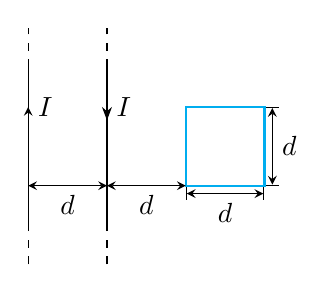
\begin{tikzpicture}[>=stealth]
                    \draw[dashed] (0,-1) -- (0,-0.5) (0,1.5) -- (0,2) (1,-1) -- (1,-0.5) (1,1.5) -- (1,2);
                    \draw[->] (0,-0.5) -- (0,1) node[right]{\(I\)};
                    \draw[arrows = {-Stealth[reversed]}] (1,-0.5) -- (1,1) node[right]{\(I\)};
                    \draw (0,0) -- (0,1.5) (1,0) -- (1,1.5);
                    \draw[cyan,thick] (2,0) rectangle (3,1);
                    \draw[<->](0,0) --node[below]{\(d\)}  (1,0);
                    \draw[<->] (1,0) --node[below]{\(d\)}  (2,0);
                    \draw[|<->|] (2,-0.1) -- node[below]{\(d\)} (3,-0.1); 
                    \draw[|<->|] (3.1,0) -- node[right] {\(d\)} (3.1,1);
                \end{tikzpicture}
                \caption{\ref{itm:7} 题图}
            \end{minipage}
            \begin{minipage}[b]{0.4\textwidth}
                \centering
                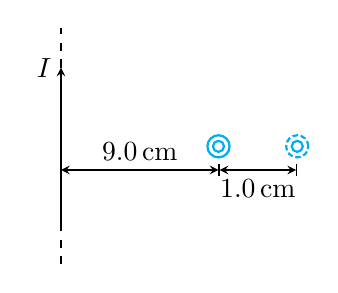
\begin{tikzpicture}[>=stealth]
                    \draw[dashed] (0,-1.5) -- (0,-1) (0,1) -- (0,1.5);
                    \draw[->] (0,-1) -- (0,1) node[left]{\(I\)};
                    \draw[cyan,thick] (2,0) circle (2pt) (2,0) circle (4pt) (3,0) circle (2pt);
                    \draw[dash pattern={on 2pt off 1pt},cyan,thick] (3,0) circle (4pt);
                    \draw[|<->|] (2,-0.3) --node[below]{\(\csi{1.0}{\cm}\)}  (3,-0.3);
                    \draw[<->] (0,-0.3) -- node[above]{\(\csi{9.0}{\cm}\)} (2,-0.3);
                \end{tikzpicture}
                \caption{\ref{itm:10} 题图}
            \end{minipage}
        \end{figure}
    \item[\mlabel{itm:10}{8-10}] 如图所示,一根长直导线中通有\(I=\csi{5.0}{\A}\)的电流,在距导线\csi{9.0}{\cm}处,放一个面积为
        \csi{0.10}{\square\cm}、10匝的小圆线圈,线圈中的磁场可看作是均匀的。今在\csi{1.0e-2}{\s}内把此线圈移至距长直导线\csi{10.0}{\cm}处。
        (1)求线圈中的平均感应电动势;(2)设线圈的电阻为\csi{1.0e-2}{\ohm},求通过线圈横截面的感应电荷。
    \item[\mlabel{itm:13}{8-13}] 如图所示,长为\(L\)的导体棒\(OP\)处于均匀磁场中,并绕\(OO^\prime\)轴以角速度\(\omega\)旋转,
        棒与转轴间的夹角恒为\(\theta\),磁感强度\(\bm{B}\)与转轴平行,求OP棒在图示位置处的电动势。
        \begin{figure}[htb]
            \centering
            \begin{minipage}[b]{0.4\textwidth}
                \centering
                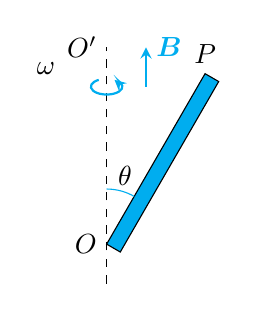
\begin{tikzpicture}[>=stealth]
                    \draw[dashed] (0,-0.5) -- (0,0) node[left]{\(O\)} -- (0,2.5) node[left]{\(O^\prime\)};
                    \draw[->,thick,cyan,yshift=2 cm] (120:0.2 and 0.1) arc (120:420:0.2 and 0.1) ;
                    \node at (0,3,2) {\(\omega\)};
                    \draw[fill=cyan,rotate=-30] (0,0) rectangle (0.2,2.5);
                    \draw[cyan] (60:0.7) arc (60:90:0.7);
                    \node at (75:0.9){\(\theta\)};
                    \draw[thick,->,cyan] (0.5,2) -- (0.5,2.5) node[right]{\(\bm{B}\)};
                    \node[above] at ({2.5*sin(30)},{2.5*cos(30)}){\(P\)};
                \end{tikzpicture}
                \caption{\ref{itm:13} 题图}
            \end{minipage}
            \begin{minipage}[b]{0.4\textwidth}
                \centering
                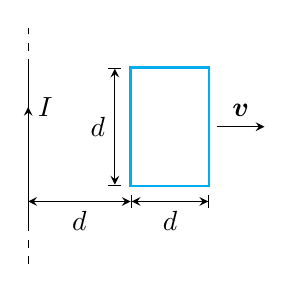
\begin{tikzpicture}[>=stealth]
                    \draw[dashed] (0,-1) -- (0,-0.5) (0,1.5) -- (0,2);
                    \draw[->] (0,-0.5) -- (0,1) node[right]{\(I\)};
                    \draw (0,0) -- (0,1.5);
                    \draw[cyan,thick] (1.3,0) rectangle (2.3,1.5);
                    \draw[<->] (0,-0.2) --node[below]{\(d\)}  (1.3,-0.2);
                    \draw[|<->|] (1.3,-0.2) --node[below]{\(d\)}  (2.3,-0.2);
                    \draw[|<->|] (1.1,0) -- node[left]{\(d\)} (1.1,1.5); 
                    \draw[->] (2.4,0.75) -- node[above]{\(\bm{v}\)} (3,0.75);
                \end{tikzpicture}
                \caption{\ref{itm:15} 题图}
            \end{minipage}
        \end{figure}
    \item[\mlabel{itm:15}{8-15}] 如图所示,在一根无限长载流直导线的近旁放置一个矩形导体线框。该线框在垂直于导线方向上以匀速率\(v\)向右移动。
        求在图示位置处线框中的感应电动势的大小和方向。
    \item[\mlabel{itm:18}{8-18}] 半径\(R=\csi{2.0}{\cm}\)的无限长直载流密绕螺线管,管内磁场可视为均匀磁场,管外磁场可近似看作零。若通电电流均匀变化,
        使得磁感强度\(\bm{B}\)随时间的变化率\(\frac{\dif B}{\dif t}\)为常量,且为正值。(1)试求管内外由磁场变化而激发的感生电场分布;(2)如
        \(\frac{\dif B}{\dif t}=\csi{0.010}{\tesla\per\second}\),求距螺线管中心轴\(r=\csi{5.0}{\cm}\)处感生电场的大小和方向。
    \item[\mlabel{itm:19}{8-19}] 在半径为\(R\)的圆柱形空间中存在着均匀磁场\(\bm{B}\),其方向与柱的轴线平行,如图所示,一根长为\(l\)的金属棒放在磁场中,
        设\(\bm{B}\)随时间的变化率\(\frac{\dif B}{\dif t}\)为常量。试证:棒上感应电动势的大小为
        \[\mathscr{E}=\frac{\dif B}{\dif t} \frac{l}{2} \sqrt{R^2-(\frac{l}{2})^2}\]
        \begin{figure}[htb]
            \centering
            \begin{minipage}[b]{0.4\textwidth}
                \centering
                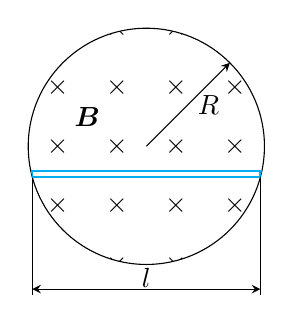
\begin{tikzpicture}[>=stealth,scale=0.75]
                    \draw[thin] (-15:2) -- ++(0,-2) (195:2) -- ++(0,-2);
                    \draw[<->] (-15:2)++(0,-1.9) -- node[above=-1mm]{\(l\)} ++({-4*cos(15)},0);
                    \clip[draw] (0,0) circle (2);
                    \foreach \x in {-1.5,-0.5,...,1.5}
                        \foreach \y in {-2.0,-1,...,2}
                            \node at (\x,\y) {\(\times\)};
                    \draw[->] (0,0) -- node[right]{\(R\)} (45:2);
                    \draw[thick,cyan] (-15:2) rectangle ++({-4*cos(15)},0.1);
                    \node at (-1,0.5) {\(\bm{B}\)};
                \end{tikzpicture}
                \caption{\ref{itm:19} 题图}
            \end{minipage}
            \begin{minipage}[b]{0.4\textwidth}
                \centering
                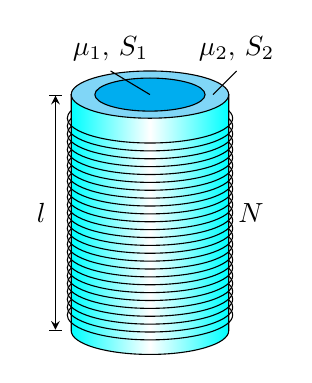
\begin{tikzpicture}[>=stealth]
                    \draw[left color=cyan, right color=cyan, middle color = white] (1,0) -- node[right]{\(N\)} ++(0,-3) arc (0:-180:1 and 0.3) -- ++(0,3) -- cycle;
                    \draw[fill=cyan!50] (0,0) ellipse (1 and 0.3);
                    \draw[fill=cyan] (0,0) ellipse (0.7 and 0.21);
                    \foreach \y in {-2.8,-2.7,...,-0.2}
                        \draw[yshift=\y cm] ({acos(1/1.05)+360}:1.05 and 0.315) arc ({acos(1/1.05)+360}:{acos(-1/1.05)}:1.05 and 0.315);
                    \draw[thin] (0,0) -- ++(-0.5,0.3) node[above]{\(\mu_1,\,S_1\)};
                    \draw[thin] (0.8,0) -- ++(0.3,0.3) node[above]{\(\mu_2,\,S_2\)};
                    \draw[|<->|] (-1.2,0) -- node[left]{\(l\)} ++(0,-3);
                \end{tikzpicture}
                \caption{\ref{itm:21} 题图}
            \end{minipage}
        \end{figure}
    \item[\mlabel{itm:21}{8-21}] 如图所示,螺线管的管心是两个套在一起的同轴圆柱体,其截面积分别为\(S_1\)和\(S_2\),磁导率分别为\(\mu_1\)和\(\mu_2\),
        管长为\(l\),匝数为\(N\),求螺线管的自感(设管的截面积很小)。
    \item[\mlabel{itm:23}{8-23}] 如图所示,在一个柱形纸筒上绕有两组相同线圈\(AB\)和\(A^\prime B^\prime\),每个线圈的自感均为\(L\),求:(1)\(A\)
        和\(A^\prime\)相接时,\(B\)和\(B^\prime\)间的自感\(L_1\);(2)\(A^\prime\)和\(B\)相接时,\(A\)和\(B^\prime\)间的自感\(L_2\).
        \begin{figure}[htb]
            \centering
            \begin{minipage}[b]{0.4\textwidth}
                \centering
                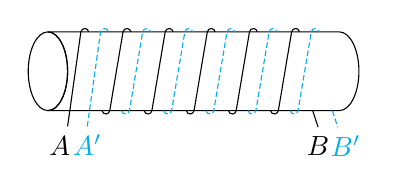
\begin{tikzpicture}[>=stealth]
                    \draw (0,0) ellipse (0.25 and 0.5);
                    \draw (0,0.5) -- ++(3.7,0) arc (90:-90:0.25 and 0.5) -- ++(-3.7,0) arc (-90:90:0.25 and 0.5) --cycle;
                    \draw (0.25,-0.7) node[below,xshift=-1mm]{\(A\)} -- ++({1.2*tan(8)},1.2) arc (172:8:0.05) coordinate (a1);
                    \draw[cyan,dash pattern={on 2pt off 1pt}] (0.5,-0.7) node[below,yshift=0.5pt]{\(A^\prime\)} -- ++({1.2*tan(8)},1.2) arc (172:8:0.05) coordinate (b1);
                    \foreach \x/\y in {1/2,2/3,3/4,4/5,5/6}
                    {
                        \draw ($(a\x)+({1.2*tan(8)},-1)$) arc (188:352:0.05) -- ++({1.2*tan(8)},1) arc (172:8:0.05) coordinate(a\y);
                        \draw[cyan,dash pattern={on 2pt off 1pt}] ($(b\x)+({1.2*tan(8)},-1)$) arc (188:352:0.05) -- ++({1.2*tan(8)},1) arc (172:8:0.05) coordinate(b\y);
                    }
                    \draw ($(a6)+({1.2*tan(8)},-1)$) -- ++(-72:0.22) node[below]{\(B\)};
                    \draw[cyan,dash pattern={on 2pt off 1pt}] ($(b6)+({1.2*tan(8)},-1)$) -- ++(-72:0.22) node[below,xshift=1mm,yshift=0.5pt]{\(B^\prime\)};
                \end{tikzpicture}
                \caption{\ref{itm:23} 题图}
            \end{minipage}
            \begin{minipage}[b]{0.4\textwidth}
                \centering
                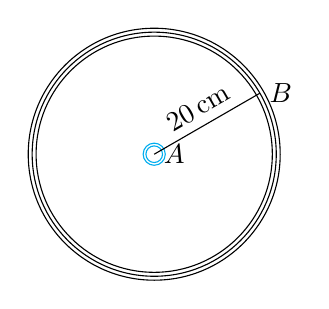
\begin{tikzpicture}[>=stealth]
                    \draw[cyan] (0,0) node[right,black]{\(A\)} circle (3pt) (0,0) circle (4pt);
                    \draw (0,0) circle (1.5) (0,0) circle (1.55) (0,0) circle (1.60);
                    \draw (0,0) -- node[above,rotate=30]{\(\csi{20}{\cm}\)} (30:1.55) node[right]{\(B\)};
                \end{tikzpicture}
                \caption{\ref{itm:24} 题图}
            \end{minipage}
        \end{figure}
    \item[\mlabel{itm:24}{8-24}] 如图所示,一个面积为\csi{4.0}{\cm\squared}共50匝的小圆形线圈A,放在半径为\csi{20}{\cm}共100匝的大圆形线圈B的正中央,
        两个线圈同心且同平面。设线圈A内各点的磁感强度可看作是相同的。求:(1)两个线圈的互感;(2)当线圈B中电流的变化率为\csi{-50}{\ampere\per\second}
        时,线圈A中感应电动势的大小和方向。
    \item[8-27] 一个直径为\csi{0.01}{\m}、长为\csi{0.1}{\m}的长直密绕螺线管,共1\,000匝线圈,总电阻为\csi{7.76}{\ohm}。问:(1)如把线圈接到电动势
        \(\mathscr{E}=\csi{2.0}{\V}\)的电池上,电流稳定后,线圈中所贮存的磁能是多少?磁能密度是多少?*\negthickspace(2)从接通电路时算起,要使线圈贮存的磁能为最大时
        的一半,需经过多少时间?
    \item[8-28] 一根无限长直导线,截面各处的电流密度相等,总电流为\(I\)。试证:每单位长度导线内所贮存的磁能为\(\frac{\mu I^2}{16\uppi}\)。
    \item[8-33] 设半径\(R=\csi{0.20}{\m}\)的平行平板电容器,两极板之间为真空,极板间距离\(d=\csi{0.50}{\cm}\)。现以恒定电流\(I=\csi{2.0}{\ampere}\)对
        电容器充电,求位移电流密度(忽略平板电容器边缘效应,设电场是均匀的)。
    \item \label{itm:s1}只有一根辐条的轮子在均匀外磁场\(\bm{B}\)中转动,轮轴与\(\bm{B}\)平行,如图所示,轮子和辐条都是导体辐条长为\(R\),轮子每秒转\(N\)圈。
        两根导线\(a\)和\(b\)通过各自的刷子分别与轮轴和轮边接触。(1)求\(a\)、\(b\)间的感应电动势;(2)若\(a\)、\(b\)间接了一个电阻,使得辐条中
        的电流为\(I\),问\(I\)的方向如何?(3)求这时磁场作用在辐条上的力矩的大小和方向;(4)当轮反转时,\(I\)是否也会反向?
        (5)若轮子的辐条是对称的两根或多根,结果如何?
        \begin{figure}[htb]
            \centering
            \begin{minipage}[b]{0.4\textwidth}
                \centering
                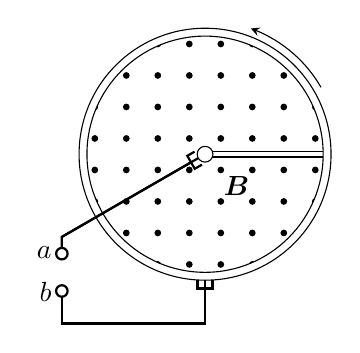
\begin{tikzpicture}[>=stealth]
                    \draw[thick,arrows={-Circle[open]}] (210:0.1) -- ++(210:2) -- ++(0,-0.3) coordinate (a1) node[left,yshift=1mm]{\(a\)};
                    \draw[thick,arrows={Bracket[reversed,inset=3pt]-}] (210:0.1) -- ++(210:2);
                    \draw[thick,arrows={Circle[open]-}] ($(a1)+(0,-0.3)$) node[left,yshift=-1mm]{\(b\)} -- ++(0,-0.5) -| (-90:1.6);
                    \draw[thick,arrows={Bracket[reversed,inset=3pt]-}] (-90:1.6) -- ++(0,-0.1);
                    \node at (0.4,-0.4) {\(\bm{B}\)};
                    \draw[->] (30:1.7) arc (30:70:1.7);
                    \draw (0,0) circle (1.6);
                    \clip[draw] (0,0) circle (1.5);
                    \foreach \x in {-1.8,-1.4,...,1.8}
                        \foreach \y in {-1.8,-1.4,...,1.8}
                            \draw[fill] (\x,\y) circle (1pt);
                    \draw (0,-1pt) rectangle (1.6,1pt);
                    \draw[fill=white] (0,0) circle (0.1);
                \end{tikzpicture}
                \caption{\ref{itm:s1} 题图}
            \end{minipage}
            \begin{minipage}[b]{0.4\textwidth}
                \centering
                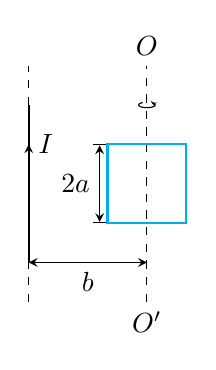
\begin{tikzpicture}[>=stealth]
                    \draw[dashed] (0,-1) -- (0,-0.5) (0,1.5) -- (0,2) (1.5,-1) node[below]{\(O^\prime\)} -- (1.5,2) node[above]{\(O\)};
                    \draw[->] (0,-0.5) -- (0,1) node[right]{\(I\)};
                    \draw[thick] (0,-0.5) -- (0,1.5);
                    \draw[cyan,thick] (1,0) rectangle (2,1);
                    \draw[<->](0,-0.5) --node[below]{\(b\)}  ++(1.5,0);
                    \draw[|<->|] (0.9,0) -- node[left]{\(2a\)} ++(0,1); 
                    \draw[arrows = {-Stealth[length=2pt]},xshift=1.5cm,yshift = 1.5cm] (120:3pt and 1pt) arc (120:420:3pt and 1pt);
                \end{tikzpicture}
                \caption{\ref{itm:s2} 题图}
            \end{minipage}
        \end{figure}
    \item \label{itm:s2} 如图所示,电流为\(I\)的长直导线附近有正方形线圈绕中心轴\(OO^\prime\)以角速度\(\omega\)旋转,求线圈中的感应电动势。
        已知正方形边长为\(2a\),\(OO^\prime\)轴与长直导线平行,相距为\(b\)。
    \item \label{itm:s3} 闭合线圈共用\(N\)匝,电阻为\(R\),证明:当通过这线圈的磁通量改变\(\Delta \varPhi\)时,线圈内流过的电荷量为
        \(\Delta q=\frac{N\Delta \varPhi}{R}\)。
    \item \label{itm:s4}一密绕的螺线环,单位长度的匝数为\(n=\csi{2000}{\per\m}\),环的横截面积为\(s=\csi{10}{\cm\squared}\),另一个\(N=10\)匝
        的小线圈套绕在环上,如图所示。(1)求两个线圈间的互感;(2)当螺线环中的电流变化率为\(\frac{\dif I}{\dif t}=\csi{10}{\ampere\per\second}\)
        时,求在小线圈中产生的互感电动势的大小。
        \begin{figure}[htb]
            \centering
            \begin{minipage}[b]{0.3\textwidth}
                \centering
                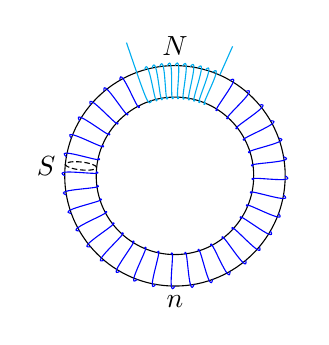
\begin{tikzpicture}[>=stealth]
                    \draw (0,0) circle (1);
                    \draw (0,0) circle (1.4);
                    \foreach \x in {30,40,...,330}
                        \draw[rotate=\x,blue] (90:1.4) .. controls (86:1.6) and (91:0.85) .. (87:1);
                    \foreach \x in {-20,-16,...,16}
                        \draw[rotate=\x,cyan] (90:1.4) .. controls (86:1.6) and (91:0.85) .. (87:1);
                    \draw[rotate=20,cyan] (90:1.8) .. controls (91:0.95) .. (87:1);
                    \draw[rotate=-24,cyan] (90:1.4) -- (90:1.8);
                    \node at (90:1.4) [above] {\(N\)};
                    \node at (-90:1.4) [below] {\(n\)};
                    \draw[dash pattern={on 2pt off 1pt},xshift=-1.2cm,rotate around={-6:(1.2,0)}] (0,0) node[left=2mm]{\(S\)} ellipse (0.2 and 0.05);
                \end{tikzpicture}
                \caption{\ref{itm:s4} 题图}
            \end{minipage}
            \begin{minipage}[b]{0.6\textwidth}
                \centering
                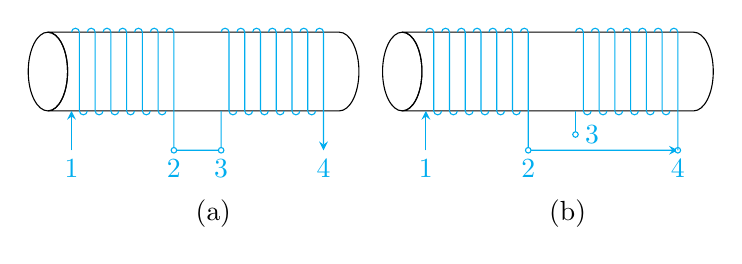
\begin{tikzpicture}[>=stealth]
                    \draw (0,0) ellipse (0.25 and 0.5);
                    \draw (0,0.5) -- ++(3.7,0) arc (90:-90:0.25 and 0.5) -- ++(-3.7,0) arc (-90:90:0.25 and 0.5) --cycle;
                    \foreach \x in {0.3,0.5,...,1.4,2.2,2.4,...,3.3}
                        \draw[xshift=\x cm,cyan] (0,0.5) arc (180:0:0.05) -- ++(0,-1) arc (180:360:0.05);
                    \draw[->,cyan] (0.3,-1) node[below]{1} -- ++(0,0.5);
                    \draw[xshift=1.5 cm,cyan] (0,0.5) arc (180:0:0.05) -- ++(0,-1.5) node[below]{2} -- ++(0.6,0) node[below]{3} -- ++(0,0.5);
                    \draw[fill=white,draw = cyan] (1.6,-1) circle(1pt) (2.2,-1) circle(1pt);
                    \draw[xshift=3.4 cm,->,cyan] (0,0.5) arc (180:0:0.05) -- ++(0,-1.5) node[below]{4};
                    \node at (2.1,-1.5)[below] {(a)};
                    \begin{scope}[xshift=4.5 cm]
                        \draw (0,0) ellipse (0.25 and 0.5);
                        \draw (0,0.5) -- ++(3.7,0) arc (90:-90:0.25 and 0.5) -- ++(-3.7,0) arc (-90:90:0.25 and 0.5) --cycle;
                        \foreach \x in {0.3,0.5,...,1.4,2.2,2.4,...,3.3}
                            \draw[xshift=\x cm,cyan] (0,0.5) arc (180:0:0.05) -- ++(0,-1) arc (180:360:0.05);
                        \draw[->,cyan] (0.3,-1) node[below]{1} -- ++(0,0.5);
                        \draw[xshift=1.5 cm,->,cyan] (0,0.5) arc (180:0:0.05) -- ++(0,-1.5) node[below]{2} -- ++(1.9,0);
                        \draw[cyan] (2.2,-0.5) -- ++(0,-0.3);
                        \draw[fill=white,draw = cyan] (1.6,-1) circle(1pt) (3.5,-1) circle(1pt) (2.2,-0.8) node[cyan,right]{3} circle(1pt);
                        \draw[xshift=3.4 cm,cyan] (0,0.5) arc (180:0:0.05) -- ++(0,-1.5) node[below]{4};
                        \node at (2.1,-1.5)[below] {(b)};
                    \end{scope}
                \end{tikzpicture}
                \caption{\ref{itm:s5} 题图}
            \end{minipage}
        \end{figure}
    \item \label{itm:s5}如图所示,两线圈的自感系数分别为\(L_1\)与\(L_2\),它们之间的互感系数为\(M\)。试求两线圈串联(a)和(b)两种情况下等效的
        总自感系数\(L\)。
    \item \label{itm:s6}一平行板电容器的两极板都是半径为\csi{5.0}{\cm}的圆导体片,在充电时,其中电场强度的变化率为\(\frac{\dif E}{\dif t}=\csi{E12}{\V\per\m\per\s}\)。
        求(1)两极板间的位移电流;(2)极板边缘的磁感应强度。
    \item 太阳每分钟垂直射于地球表面上每\csi{}{\cm\squared}的能量约为2\,cal(\(1\,\textmd{cal}\approx\csi{4.2}{\joule}\)),
        求地面上日光中电场强度\(E\)和磁场强度\(H\)的方均根值。
\end{enumerate}
\end{document} 